\section{Model-Based Clinical Trials}
The final step before the introduction of a new high-risk medical device to market is the \emph{clinical trial}.
The \emph{randomized controlled trial} (RCT) is the ``gold standard'' for guaranteeing that a medical intervention is safe and efficacious \cite{FriedmanFD10_ClinicalTrials}.
It is in general a major effort involving patients, medical investigators, biostatisticians, ethics boards,  regulators and companies, costing several millions of dollars and running for 4-6 years on average.
Yet technical errors can arise at almost every step of the trial planning, jeopardizing the validity of the results. 
Even if the trial is well-planned, poor execution, unexpected events or even just pure chance can lead to the wrong conclusions.
The applications of computer models to the medical domain presented above have largely centered on the design and verification of a given device, and have mostly eschewed matters related to the clinical trial.
There is however now an opportunity to use these computer models to assist in the planning and conduct of RCTs, as will be presented in this section.
(Another application of modeling to trials is the UVA/PADOVA diabetes model, which replaces \emph{animal} trials for evaluating diabetes control algorithms \cite{pancreas_paul}). 

Suppose that a manufacturer of medical devices is designing a new implantable defibrillator for the treatment of certain abnormal cardiac rhythms, or \emph{arrhythmias}.  
Both the hardware and software are tested by the company to ensure they satisfy their specifications.
The device may then be implanted and tested on animals. 
But up to this point, the effect of the device on humans has not been observed. 
%Observations of interest extend beyond whether the device operates as intended or not to whether it can be implanted safely, whether it has unexpected side effects, and whether it treats the targeted arrhythmias better than current medical care.
The RCT compares the efficacy and safety of the device on two groups of patients: the \emph{treatment group} which is implanted with the new investigational device, and the \emph{control group} which is on standard medical care, e.g. one or more devices already on the market~\cite{FriedmanFD10_ClinicalTrials}.
%The assignment of a patient to the treatment or control group is done \emph{at random}, which guarantees the validity of the statistical tests used to analyze the results and helps ensure that the two groups are comparable.
Both treatment and control groups are monitored for a pre-determined amount of time, at the end of which the rate of treated arrhythmias is evaluated in each group. The results are analyzed to determine whether the difference in rates between the groups, if any, is \emph{significant}, i.e. is unlikely to be due to chance alone.

%We call this the Model-Based Clinical Trial (MBCT). 
%Broadly speaking, we define an MBCT to be a trial in which the subjects are \emph{computer models of the physiological phenomena being studied, including the effect of the device}, rather than humans. 
%An MBCT allows us to run very large-scale targeted simulated trials to better inform our conduct of an actual RCT. 


We can design a \emph{Model-Based Clinical Trial} (MBCT) to test a number of assumptions made by the trial investigators, before the trial starts (Fig.~\ref{fig:mbct}).
In an MBCT, we start by modeling the physiological phenomenon of interest, in this case the spread of electrical activity in the human heart.
The model should be valid of course (i.e., not produce too many non-physiological signals).
For an MBCT the model must also be \emph{rich}: it should be capable of simulating a large variety of arrhythmias that are targeted by the new defibrillator.
Once such a parametrized model is created, we can generate a large number of model instances by sampling the parameter space from appropriate distributions, which may be inferred from previous trials' data.
This constitutes our synthetic cohort. 



We can now analyze the effect of the device in ways not possible or impractical with a clinical trial, so as to guide the RCT investigators when designing the trial's protocol.
For example, we may vary the distribution of arrhythmias in our synthetic cohort and analyze how this affects the device's performance. 
This is equivalent to running multiple trials on different populations in which the arrhythmias appear in different proportions.
The investigators can then use these results to confirm or revise their confidence in the superiority of the new device to standard medical care across populations.
We can also study the sensitivity of the trial's outcome to device settings: by running the trial multiple times with the same synthetic cohort but with different device settings every time, we get solid estimates for how different settings affect the MBCT's outcome. 
This in turn can inform the investigators whether they need to correct for different settings when drawing the trial protocol and when analyzing the results.
Further, by breaking down the MBCT results by arrhythmia (or other interesting criteria) the investigators can make informed decisions, before trial start, on which classes of arrhythmias are most or least susceptible to treatment by the device.
This in turn helps refine the eligibility criteria and focus the trial's efforts on certain classes of patients. 

	
This and other experiments possible in an MBCT increase the probability of success of an RCT by providing early, fast and rigorous testing of various assumptions and hypotheses made by the trial investigators.
%\yhl{For example, for a trial on implantable defibrillators, we can study how variations in a patient's physiological parameters, like speed of propagation of the electric current in the heart, affects the safety and efficacy of the device. 
%This provides valuable insight into which patients should be enrolled in the trial (and in whom the device is most efficacious).
%Another application is to get tighter estimates of statistical quantities like effect size needed before the conduct of the trial.
%A poor effect size estimate leads to a poor sample size estimate, with a real risk of the trial not yielding significant results even if there's a true meaningful difference between treatment and control.
%Yet a third application is to test how changing device settings affects the outcome of interest. 
%This is an example of an experiment ideally suited for model-based investigation, since we can connect the same heart models to the device under all settings, which is typically not possible with real patients.}
%
%\yhl{The Model-Based Clinical Trial promises to usher in a new era in clinical trials planning and medical device development in general, where the trial investigators can quickly, cheaply and reliable assess various assumptions, in ways that are not always feasible in a real trial. 
%A key component of an MBCT is the model.}
%We start with a parametrized model of the heart.
%For the model to be interpretable by physicians, it is important that the parameters have physiological significance, e.g., the refractory periods of the AV node.
%Thus physiological ranges for the parameters are known.

\begin{figure}[t]
	\centering
	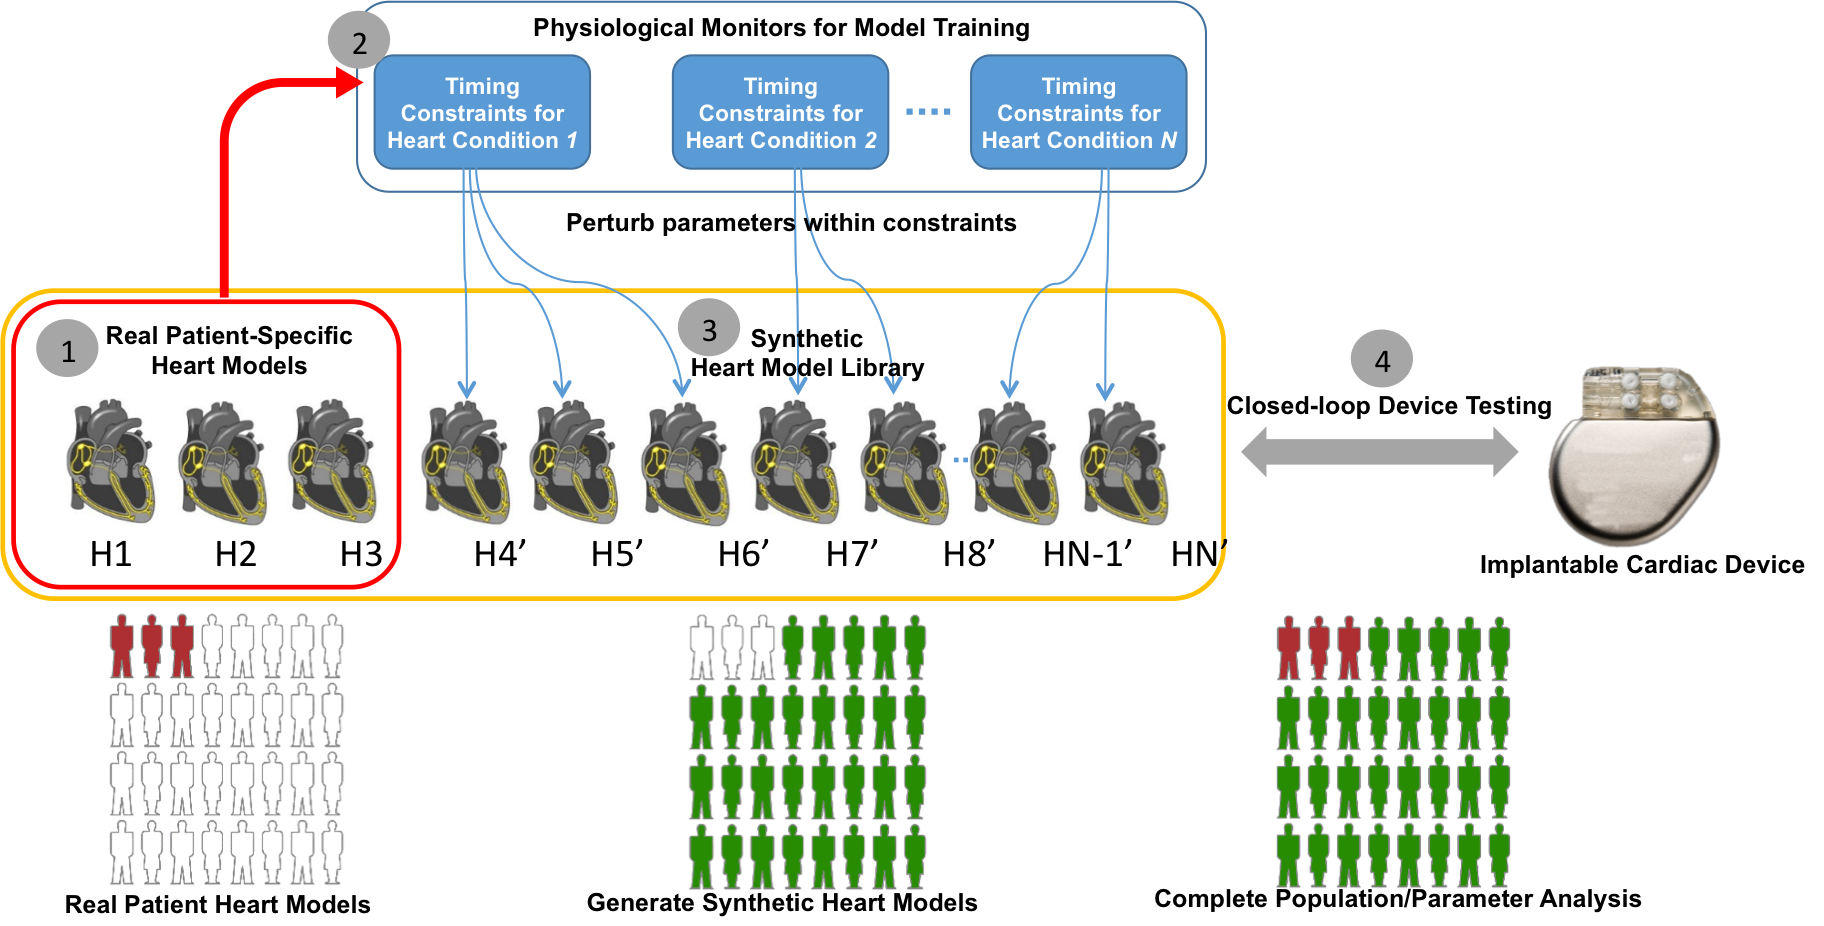
\includegraphics[width=\textwidth]{figs/fig5mbct.png}
	\caption{\small Model-based Clinical Trials. The synthetic cohort is generated by randomizing a parametrized model from an appropriate distribution whose bounds are inferred from clinical data. The parameters are sampled within their physiological ranges, thus generating a large synthetic cohort. Each such model instance is connected to the device and simulated.}
	\label{fig:mbct}
\end{figure}

%Early efforts tying physiological modeling to clinical trials include the UVA/PADOVA diabetes model which is used to generate simulated patients.
%New diabetes control algorithms are evaluated on simulated patients instead of animals to assess their efficacy. These applications of MBCT usher a new era of exciting research challenges for the closed-loop verification, validation and testing medical devices at scale. MBCT have the potential to reduce the scope, cost and probability of failure of clinical trials of medical devices with complex hardware and software. MBCT when viewed as a rapid certification toolchain to speed up medical device approvals is  gaining increasing traction both within the regulatory environment and the medical device industry.
\section{Conclusion}

This article has surveyed the challenges of bringing new medical devices and their software to market from early verification to late-stage clinical trials, and gives an outlook to how modeling and formal methods can play a role in facilitating this process.
\emph{Complexity, limited observability and variability} stand out as three major challenges.
The \emph{complexity} of the physiological phenomena that the device is meant to control stems partially from the multi-scale nature of human physiology, where an organ's operation is affected by both molecular factors and patient's lifestyle.
Moreover, the devices have limited \emph{observability} on these complex physiological phenomena because increased observability usually requires increased invasiveness of the surgical procedures, with all the attending risks.
%Thus, an implantable defibrillator currently has only three contact points with the myocardium, from which it tries to infer the nature of the global electrical activity.
Coupled together, complexity and limited observability imply that the detection and therapy algorithms of devices must deal, safely and reliably, with a lot of uncertainty.
By explicitly allowing for non-determinism in the systems they study, formal methods are well-suited for dealing with uncertainty.
The major challenge for formal methods is the development of appropriate physiological models and abstraction-and-refinement frameworks for addressing the complexity of the phenomena, and abstraction trees take a step in this direction in the domain of electrophysiology.
\emph{Variability} arises as the third major challenge: how to verify that a device works well in a population of patients that varies greatly in its characteristics and medical history?
Clinical trials remain the standard and legally accepted way to answer that question.
While models can not substitute for observations in a human patient, they promise to alleviate the burden of conducting trials by early and rigorous testing of their assumptions.
These applications usher a new era of exciting research challenges at the intersection of computer science, statistics and medicine.
